\documentclass{article}
\usepackage[final]{neurips}
\usepackage[framemethod=tikz]{mdframed}
\usepackage{lipsum}
\definecolor{mycolor}{rgb}{0.122, 0.435, 0.698}
\newmdenv[innerlinewidth=0.5pt, roundcorner=4pt,linecolor=mycolor,innerleftmargin=6pt,
innerrightmargin=6pt,innertopmargin=6pt,innerbottommargin=6pt]{mybox}
\usepackage[utf8]{inputenc} % allow utf-8 input
\usepackage[T1]{fontenc}    % use 8-bit T1 fonts
\usepackage[hidelinks]{hyperref}       % hyperlinks
\usepackage{url}            % simple URL typesetting
\usepackage{booktabs}       % professional-quality tables
\usepackage{amsfonts}       % blackboard math symbols
\usepackage{nicefrac,tcolorbox}       % compact symbols for 1/2, etc.
\usepackage{amsmath}
\usepackage{enumitem}
\usepackage{microtype}      % microtypography
\usepackage{graphicx,caption}
\usepackage{xepersian}
\settextfont{XB Niloofar}
\setdigitfont{XB Niloofar}
\raggedbottom


\title{
	\vspace{-0.8em}
تمرین سری دوم درس نظریه گروه‌ها - دکتر رضاخانی
\\
{\normalsize
\textbf{مهلت تحویل:
جمعه ۲۵ اسفند ماه سال ۱۴۰۲ تا ساعت 59:23
\\
\vspace{-0.4em}
از طریق سامانه
\href{https://cw.sharif.edu/}{درس‌افزار شریف}
}
}
\vspace{-0.6em}
}

\usepackage[utf8]{inputenc}

\usepackage[english]{babel}
\setlength{\parindent}{3.5em}
\setlength{\parskip}{0.5em}
\renewcommand{\baselinestretch}{1.0}

\usepackage{calrsfs}
\DeclareMathAlphabet{\pazocal}{OMS}{zplm}{m}{n}
\newcommand{\La}{\mathcal{L}}
\newcommand{\Lb}{\pazocal{L}}

\newtcolorbox{boxes}[3][]
{
	colframe = #2!25,
	colback  = #2!10,
	coltitle = #2!40!black,  
	title    = {\textbf{#3}},
	#1,
}

\newenvironment{exercise}[3][\unskip]{%
	\par
	\noindent
	\textbf{تمرین
		#1
		[#2 امتیاز] 
		\def\temp{#3}\ifx\temp\empty
		: 
		\else
		: #3 \vspace{0.5em} \\ \noindent
		\fi
}}{}

\author{
حسین محمدی\\
  \lr{
  		\href{mailto:hossein.mohammadi.00427@gmail.com}{\texttt{	hossein.mohammadi.00427@gmail.com}}} \\
  \And
  زهرا کبیری\\
 \lr{
  		\href{mailto:kabiri.zahra98@gmail.com}{ \texttt{kabiri.zahra98@gmail.com}}}\\
  }

\begin{document}


\begin{minipage}{0.1\textwidth}% adapt widths of minipages to your needs
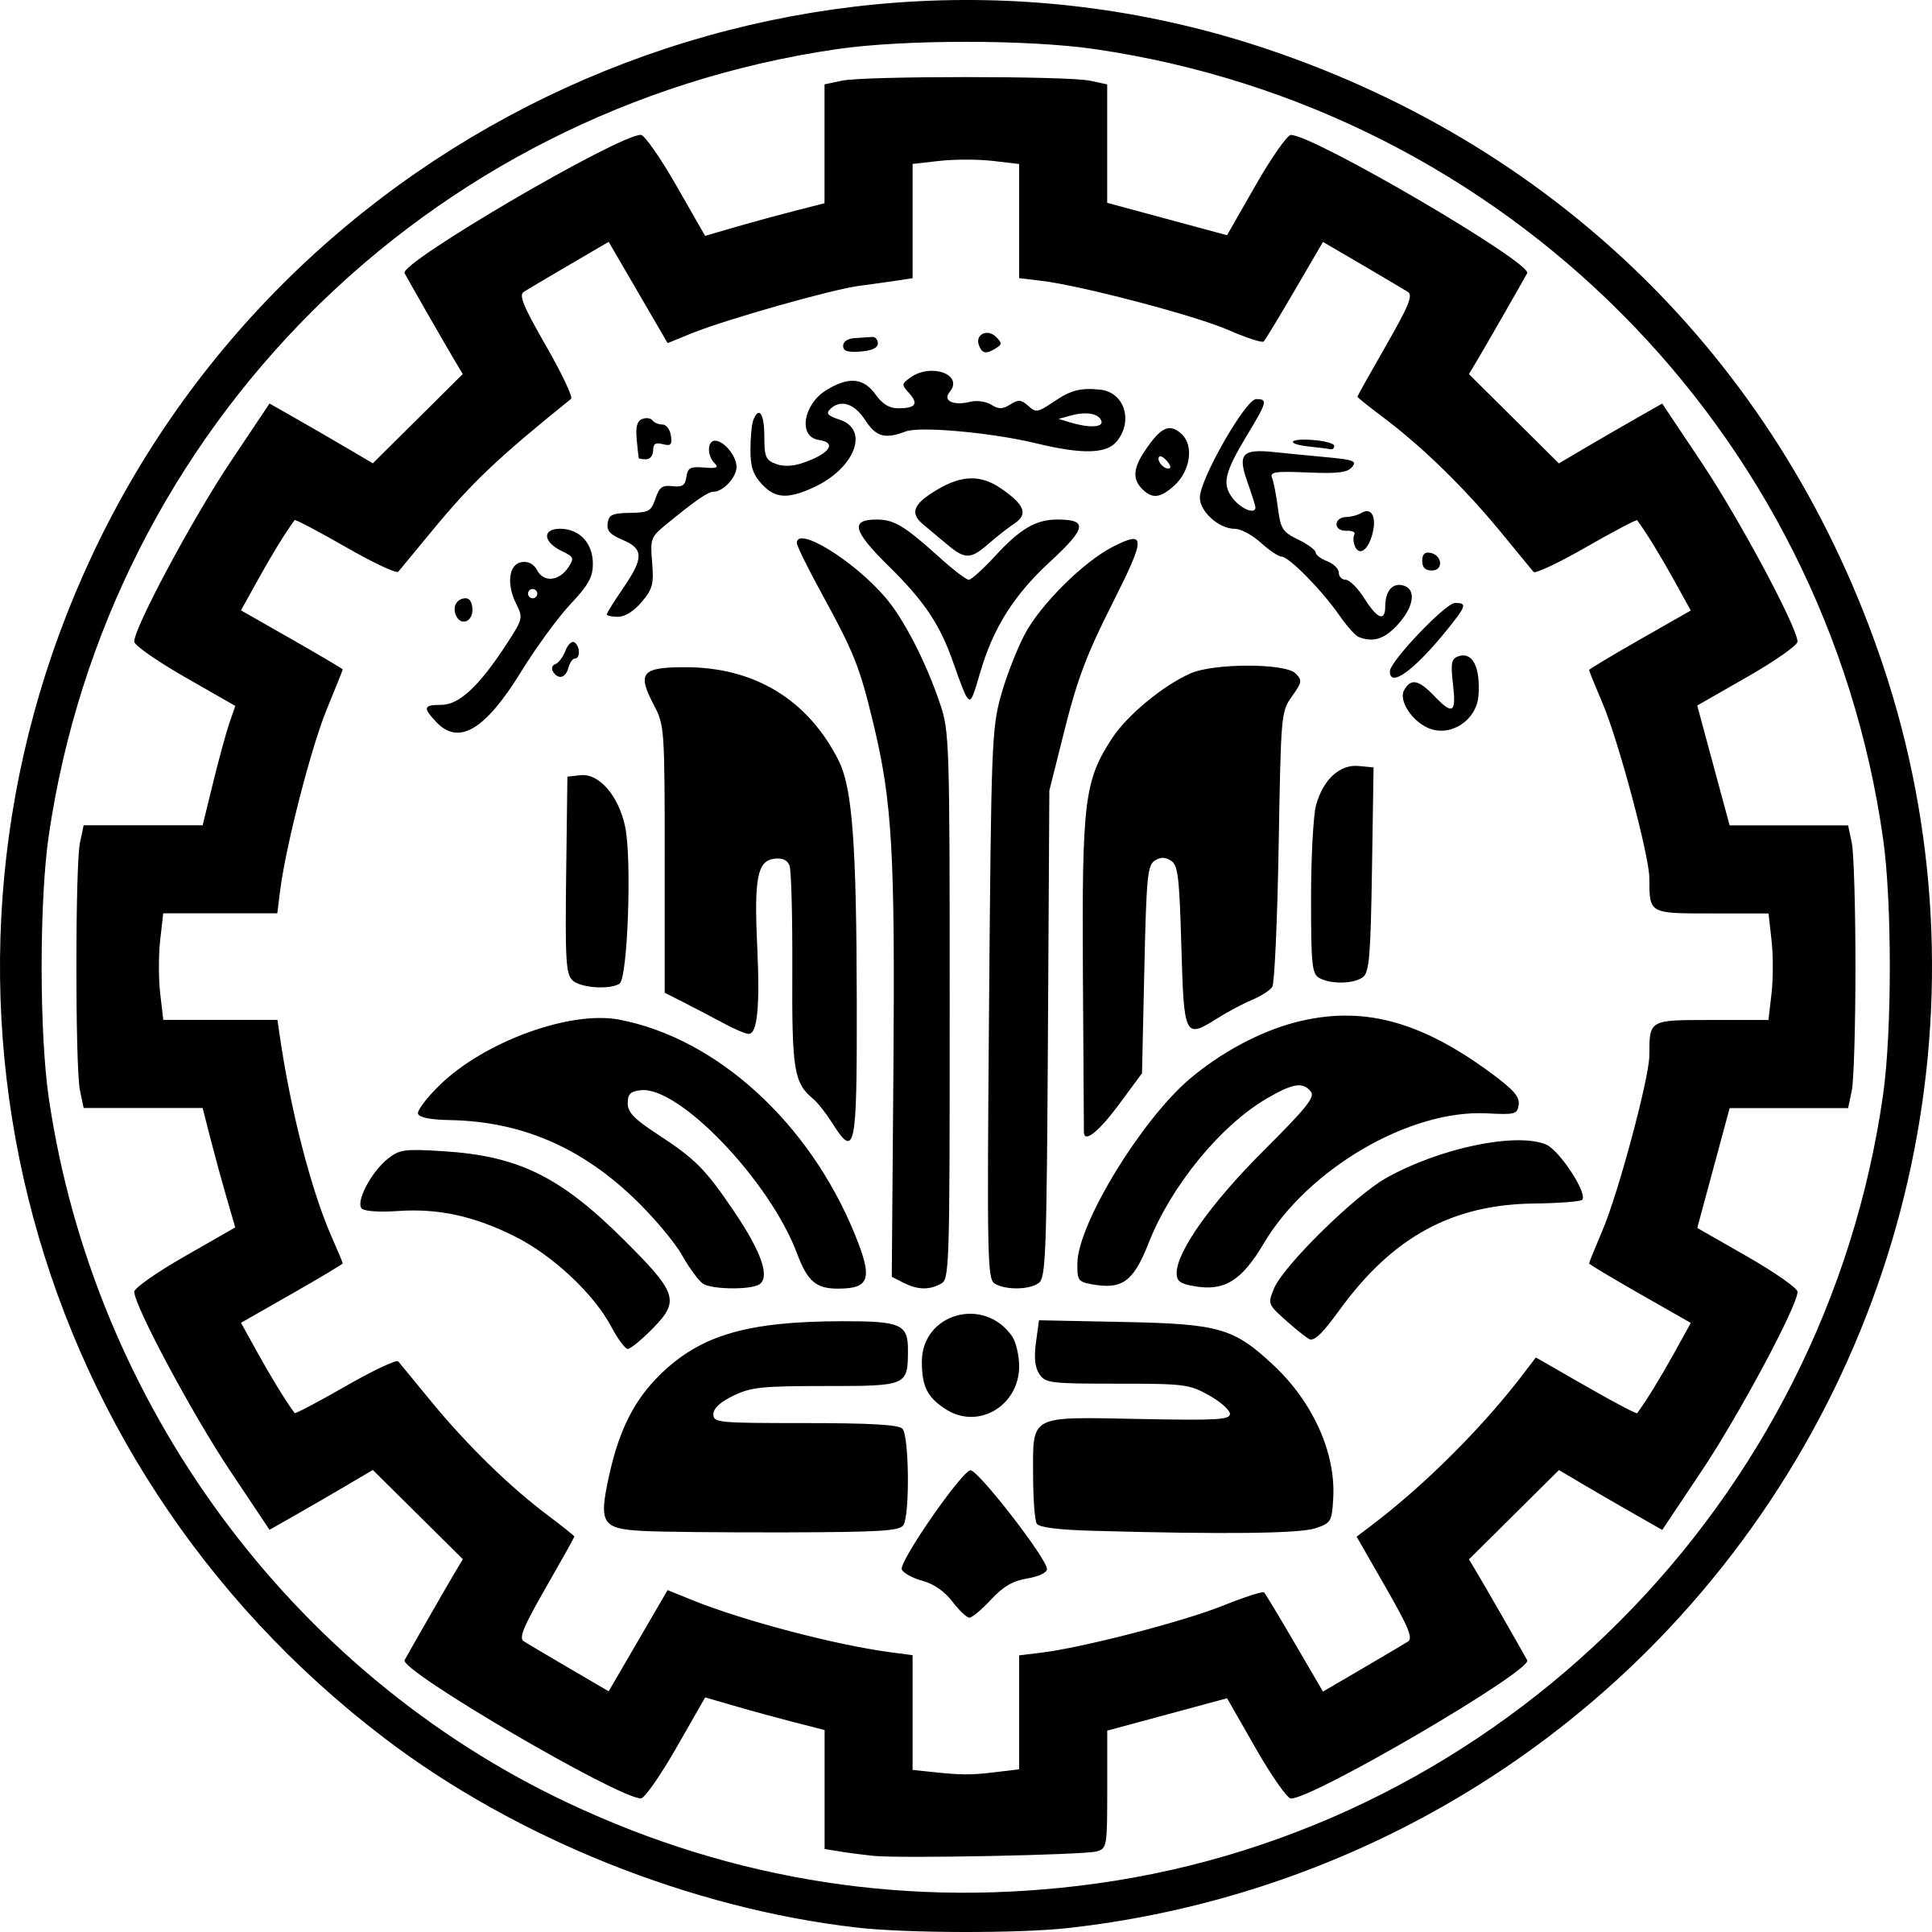
\includegraphics[width=1.1cm]{sharif-logo.png}
\end{minipage}%
\hfill%
\begin{minipage}{0.9\textwidth}\raggedleft
دانشگاه صنعتی شریف\\
زمستان ۱۴۰۲ - بهار ۱۴۰۳\\
\end{minipage}

\makepertitle


\begin{exercise}[۶]{20}{همریختی و یکریختی و خواصشان}
	با همریختی و یکریختی در کلاس آشنا شدید، بیاید آشنایی‌مان را گسترش بدهیم. فرض کنید دوگروه 
	$(G,.)$
	و
	$(H,*)$
	مفروض‌اند و همسانی
	$\phi: G \to H$
	بین این دوگروه داده ‌شده‌است.
	
	\vspace{0.5em}
	\noindent
	الف) نشان دهید که 
	$\phi$
	عضو خنثای گروه 
	$G$ را به عضو خنثای گروه 
	$H$ می‌برد؛ یعنی 
	$\phi(e_G) = e_H$.
	
	\noindent
	ب) نشان دهید وارون هر عضو 
	$g \in G$ 
	به وارون تصویرش نگاشته می‌شود:
	$\phi(g^{-1}) = \phi(g)^{-1}$.
	
	\noindent
	ج) در سری قبلی با مرتبه‌ی یک عضو از گروه آشنا شدید. آیا همسانی لزوما مرتبه‌ی اعضای گروه را حفظ می‌کند؟ برای حرف خود اثبات یا مثالی ارائه کنید
	\footnote{لطفا از مثالهای بدیهی برحذر باشید و به‌دنبال نمونه‌های جالب‌تر باشید.}
	.
	
	\noindent
	د) اگر نگاشت 
	$\phi$
	یکسانی باشد، پاسخ شما به سوال قبل (قسمت ج) چه تغییری می‌کند؟ برای ادعای خود اثبات یا مثالی ارائه کنید. 
	
	\noindent
	ح) نشان دهید هسته‌ی همسانی $\phi$ تشکیل یک زیرگروه از $G$ می‌دهد؛ همچنین بررسی کنید که آیا تصویر نگاشت $\phi$ در گروه $H$ یک زیرگروه است.
	\setlength{\abovedisplayskip}{0pt} \setlength{\belowdisplayskip}{0pt} \setlength{\abovedisplayshortskip}{0pt} \setlength{\belowdisplayshortskip}{0pt}
	\[
	\text{Ker}\; \phi = \{ g\in G \big| \phi(g) = e_H\}
	\]
	
	
\end{exercise}

\vspace{1em}
\begin{exercise}[۷]{20}{مثالهایی از همریختی و یکریختی}
	\noindent
	الف) نشان دهید گروه جایگشت‌های سه شی $S_3$ با گروه سه‌وجهی $D_3$ (که گروه تقارنی مثلث متساوی‌الاضلاع است)، یکریخت است؛ می‌نویسیم 
	$S_3 \cong D_3$.
	برای اینکار کافی است بگویید که نگاشت مذکور، اعضای این دو گروه را چطور به هم می‌نگارد و آیا نگاشتتان خواص یکریختی را دارد؟
	
	\noindent
	ب) نشان دهید گروه 
	$\mathbb{Z}_4$ 
	با گروه
	 $\mathbb{Z}_2\times \mathbb{Z}_2$ یکریخت نیست؛ برای این کار از نتایج تمرین ۱ استفاده کنید.
	
	\noindent
	ج) گروه ماتریس‌های حقیقی
	$n\times n$
	با عمل ضرب ماتریسی، 
	$GL(n,\mathbb{R})$
	و گروه اعداد حقیقی ناصفر با عمل ضرب،
	$(\mathbb{R}-\{0\},\times)$
	را در نظر بگیرید. سعی کنید همریختی‌ای از 
	$GL(n,\mathbb{R})$
	به 
	$(\mathbb{R}-\{0\},\times)$
	تعریف کنید
	\footnote{فکر کنید به چند طریق می‌توان به یک ماتریس یک عدد نسبت داد. یادتان باشد که  همریختی باید خاصیت ضرب گروهی را حفظ کند.}
	.
	
	
\end{exercise}
\vspace{1em}

%%%%%%%%%%%%%%%%%%%%%%%%%%%%%%%%%%%%%%%%%%%%%%%%%%%%%%%%%%%%%%%%%%
% Write Exerciese Here:


\begin{exercise}[۸]{35}{گروه جایگشت‌ها
	\LTRfootnote{Symmetric Group}
	}
	الف) نشان دهید که گروه $S_n$ با $(n-1)$ ترانهش
	\footnote{جایگشتی است که تنها جای دو عضو را عوض می‌کند و بقیه را تغییر نمی‌دهد. ترانهش معادل 
	\lr{Transposition}
	است.
	}
	زیر تولید می‌شود
	\footnote{
	مقصود از نمادگذاری 
	$G = \left <a_1,a_2,\dots,a_n \right >$
	این است که گروه هر عضو
 $g\in G$
 ، از ضرب 
 $a_1$
 و
 $a_2$ 
 تا $a_n$
 ساخته می‌شود. توجه کنید که این اعضا می‌توانند تکرار شوند.
 
	}
	:
	\setlength{\abovedisplayskip}{8pt} \setlength{\belowdisplayskip}{8pt} \setlength{\abovedisplayshortskip}{8pt} \setlength{\belowdisplayshortskip}{8pt}
	\[
	S_n =  \left < (12),(13),\dots,(1n) \right >
	\]
	یعنی باید نشان دهید که تمامی اعضای گروه 
	$S_n$
	به شکل حاصل ضربی از این ترانهش‌ها بازنویسی می‌شوند.
	
	\noindent
	ب) تعداد اعضایی از
	$S_n$ 
	را که ساختار دوری
	\LTRfootnote{Cycle Structure}
	مشخص دارند، بشمارید.
	
	
	\noindent
	فرض کنید در یک عضو،
	$m$
	دور داریم و  طول هرکدام از این دورها
	$\ell_i$
است(
$1 \leq i \leq m$
و 
$\sum_{i=1}^m \ell_i = n$
)؛ بنابراین این عضو ساختار دوری زیر را دارد:
\[
(i^{(1)}_1 i^{(1)}_2 \dots i^{(1)}_{\ell_1})(i^{(2)}_1 i^{(2)}_2 \dots i^{(2)}_{\ell_2})
\dots 
(i^{(m)}_1 i^{(m)}_2 \dots i^{(m)}_{\ell_m})
\]
			که به جای تک‌تک نمادهای 
			$i^{(k)}_j$
			اعداد طبیعی بین ۱ تا $n$ قرار می‌گیرند. به چند طریق می‌توان این کار را کرد و اعضای متمایز حاصل کرد؟
		
	\noindent
	ج) اگر 
	$\alpha \in S_n$
	 جایگشت دلخواهی باشد، نشان دهید که:
	 \[
	 \alpha (i_1i_2\dots i_r)\alpha^{-1} = (\alpha(i_1)\alpha(i_2)\dots \alpha(i_r))
	 \]
\end{exercise}
\begin{exercise}[۹]{25}{
		گروه‌های از مرتبه‌ی ۸ و قضیه‌ی کیلی
	}
	قضیه‌ی کیلی هر گروه متناهی $G$ با مرتبه $|G|$ را در گروه $S_{|G|} $
	می‌نشاند. در این تمرین با گروه‌های از مرتبه‌ی ۸ آشنا می‌شویم و مطابق قضیه کیلی آنها را در 
	$S_8$
	می‌نشانیم.
	
	\noindent
	پنج گروه متمایز
	\footnote{حالا با دانستن یکریختی می‌توانیم منظورمان از  «متمایز» را دقیق‌تر کنیم. دو گروه متمایزند اگر بین‌ آن‌ها یکریختی وجود نداشته باشد.}
	از مرتبه هشت داریم:
		\setlength{\abovedisplayskip}{8pt} \setlength{\belowdisplayskip}{8pt} \setlength{\abovedisplayshortskip}{8pt} \setlength{\belowdisplayshortskip}{8pt}
	\begin{enumerate}

		\item گروه 
		$\mathbb{Z}_8$
		 \item گروه
		 $\mathbb{Z}_4\times \mathbb{Z}_2$
		 \item گروه 
		  $\mathbb{Z}_2\times \mathbb{Z}_2 \times \mathbb{Z}_2$
		  \item  گروه
		  $D_4$ یا همان گروه چهاروجهی (تقارن‌های یک مربع)
		  \item گروه کواترنیون‌ها
		  \footnote{برای اطلاع بیشتر از گروه کواترنیون ها به 
		  \href{https://en.wikipedia.org/wiki/Quaternion_group}{این صفحه ویکی‌پدیا}
		  مراجعه کنید.
		  }
	\end{enumerate}
	اعضای این گروه‌ها را بنویسید. سپس به کمک اثباتی که از قضیه کیلی بلدید این گروه‌ها را در 
	$S_8$
	بنشانید. توجه کنید که فرآیند نشاندن این گروه‌ها در $S_8$ و این که هر عضو متناظر با چه عضوی در $S_8$ می‌شود باید به صراحت نوشته شده باشد.
\end{exercise}



\begin{boxes}{black}{راهنمایی در مورد نام‌گذاری نگاشت‌ها:}
	حتما به نگاشت‌های بین ساختارهای مختلف برخورده‌اید و شاید اسامی مشابهشان شما را سردرگم کرده باشد. یکریختی
	\LTRfootnote{Isomorphism}
	، همریختی
	\LTRfootnote{Homomorphism}
	، همسان‌ریختی
	\LTRfootnote{Homeomorphism}
	، تکریختی
	\LTRfootnote{Monomorphism}
	، به‌روریختی
	\LTRfootnote{Epimorphism}
	درون‌ریختی
	\LTRfootnote{Endomorphism}
	،
	خودریختی
	\LTRfootnote{Automorphism}
	
	, هموارریختی
	\LTRfootnote{Diffeomorphism}
	(گاهی وابرسانی)
	از مکررترین نوع نگاشت‌هاست. اینجا سعی می‌کنیم کمی این واژگان را روشن‌تر کنیم
	\footnote{البته این لیست همچنان ادامه دارد. حدود پنجاه واژه تخصصی هست که از ریشه 
		\lr{"morph"} 
		مشتق شده. شاید آشناترین آن برای ما 
		\lr{holomorphism}
		و
		\lr{heteromorphism}
		باشد.
	}
	.
	
	\noindent
	همانطور که معلوم هست، تمامی این واژگان در ریشه‌ی 
	\lr{"morph"}
	و پسوند 
	\lr{"ism"}
	مشترکند. ریشه‌ی \lr{"morph"} که از یونانی به زبان‌های لاتین راه‌یافته، به معنای «شکل و ریخت» است.
	
	\noindent
	کلمه‌ی 
	\lr{"Homomorphism"}
	با پیشوند 
	\lr{"homo"}
	ساخته‌شده است؛ این پیشوندِ اصالتا یونانی، معنای «همسان و هم‌سنگ» دارد؛ پس می‌توانیم این کلمه را «هم‌سانی یا همریختی» ترجمه کنیم.
	
	\noindent
	اما‌ 
	\lr{"Isomorphism"}
	از پیشوند لاتین 
	\lr{"isos"}
	به معنای‌ «معادل و یکسان» استفاده شده؛ پس ترجمه‌ی مناسب این واژه «یکریختی یا یکسانی» است.
	
	\noindent
	به همین ترتیب در سایر واژه‌ها هم از پیشوندهای مناسب برای رساندن مفهوم استفاده شده؛ اما چیزی که برای ما مهم است، تعریف فنی پنج واژه‌ای است که با آن بیشتر سروکار خواهیم داشت.
	\footnote{این واژه‌ها را در ارتباط با گروه‌ها تعریف می‌کنیم؛ در ارتباط با سایر ساختارهای جبری، اصلاحات جزئی در تعریف صورت می‌گیرد.}
	
	\noindent
	تصور کنید دو گروه 
	$(G,.)$
	و 
	$(H,*)$
	را داریم.
	
	\begin{enumerate}
		\setlength{\itemsep}{1pt}
		\setlength{\parskip}{0pt}
		\setlength{\parsep}{0pt}
		\item 
		همریختی گروهی: نگاشتی بین دو گروه است به طوری که ساختارِ عمل گروه را حفظ کند.
		\[
		\phi: G \to G \;\;\;\; : \;\;\;\; \forall g_1,g_2 \in G \;\;\;\;\;\; \phi(g_1.g_2) = \phi(g_1)*\phi(g_2)
		\]
		\item 
		تکریختی گروهی: اگر نگاشت 
		$\phi$
		علاوه بر همریختی، یک‌به‌یک هم باشد؛ در آن صورت آن را یک نگاشت تک‌ریخت می‌نامیم.
		\item 
		به‌روریختی گروهی: اگر نگاشت 
		$\phi$
		علاوه بر همریختی، به‌رو(پوشا) هم باشد؛ در آن صورت آن را یک نگاشت به‌روریخت می‌نامیم.
		\item 
		یکریختی گروهی: اگر نگاشت 
		$\phi$
		در آن واحد همریختی، تکریختی و به‌روریختی باشد
		\footnote{گاه نگاشت‌هایی را که یک‌به‌یک و پوشا هستند، دوسویی می‌گوییم.}
		، آن را یکریختی می‌گوییم.
		
		\item 
		خودریختی گروهی: اگر نگاشت 
		$\phi : G \to G$
		در آن واحد همریختی، تکریختی و به‌روریختی باشد
		، آن را خودریختی می‌گوییم.
	\end{enumerate}
	خودریختی‌ها هم به دو دسته‌ی درونی و بیرونی تقسیم می‌شوند.
	نگاشت 
	\begin{equation}
		\varphi_g (x) : G \to G \;\;\;\;,\;\;\;\;\; \varphi_g(x) = g^{-1}xg
		\label{auto}
	\end{equation}
	یک خودریختی دورنی است. هر خودریختی دیگری که به این فرم نوشته‌ نشود، خودریختی بیرونی است
	\footnote{مثلا در گروه اعداد صحیح با عمل جمع، نگاشت 
		$\varphi(m) = -m$
		یک خودریختی خارجی است. توجه کنید که چون گروه اعداد صحیح آبلی است، خودریختی‌های داخلی‌اش بدیهی می‌شود.
	}
	.
	
\end{boxes}

\newpage

 \end{document}
